\section{Konzept}

\subsection{SystemArchitektur}

Mit diesem Projekt wird Praxisruf um die Funktionen Sprachsynthese und Gegensprechanalge erweitert.
Um dies zu ermöglichen, sind Erweiterungen an der Systemarchitektur nötig.
Bestehende Module bleiben.
Modularität wird erweitert.
Bisher nur Package Trennung.
Neu werden Gradle Module pro Domain gemacht.
Immernoch in einem Service nachher.
Aber eine Stufe näher daran, es in Microservices aufzutrennen.
Übersichtlicher, einfacher erweitertbar.
Trennung der Domänen garantiert.

\begin{figure}[h]
    \centering
    \begin{minipage}[b]{0.9\textwidth}
        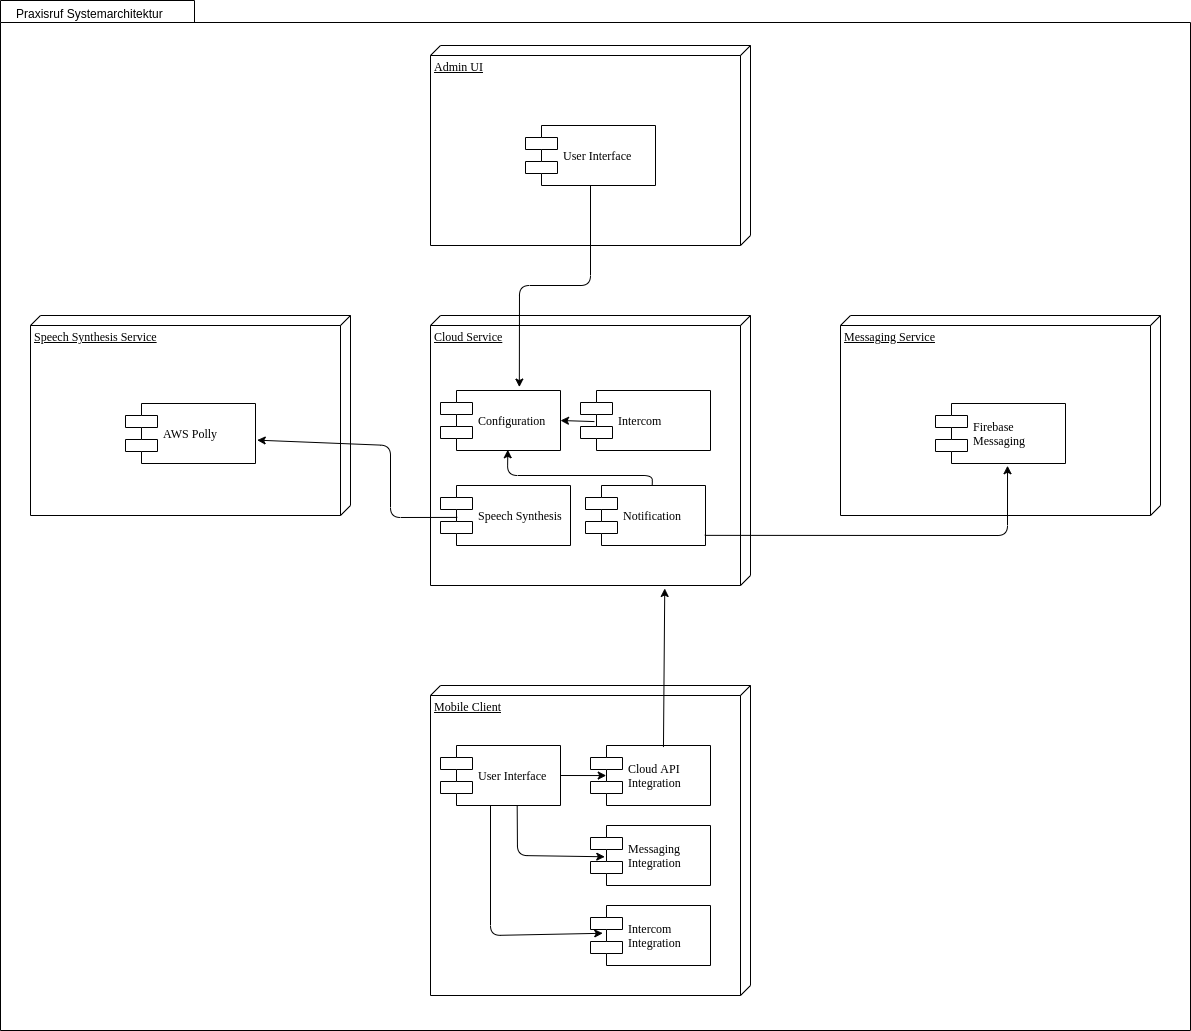
\includegraphics[width=\textwidth]{graphics/diagramms/Component_System_V01}
        \caption{Systemarchitektur Praxisruf}
    \end{minipage}
\end{figure}

\subsubsection*{Cloudservice}

Auf Seite Cloud Service werden die Module Intercom und Speech Synthesis hinzugefügt.
Intercom übernimmt das Signaling für WebRTC.
Hat den Vorteil, dass künftig auch Web und Android Clients an denselben Signaling Service angebunden werden können.
Vermittlung passiert anhand der vom Admin erfassten Konfiguration. \\

Speech Synthesis dient als einheitliche Schnittstelle zu einem externen Seepch Synthesis Service.
Dadurch kann auch wenn ein Android oder Web Client kommt, dieser genau gleich angebunden werden.
Garantie, dass die Konfiguration und Funktionsweise dieselbe für alle Clients ist. \\

\subsubsection*{Mobile Client}

Neu als nativer Client mit SwiftUI.
Beinhaltet des Benutzer Interface.
Sowie Komponenten zur Anbindung an Configuration, Notification, Speech Synthesis und Intercom.
Details in Client Kapitel. \\

\subsubsection*{Admin UI}
Das Admin UI dient weiterhin zur Administaration der Configuration.
Das Admin UI wird um Konfigurationsmöglichkeiten für Speech Synthesis und Gegensprechanalge werweitert. \\


\subsubsection*{Speech Synthesis Service}
Als neuer externer Service AWS Polly angebunden.
Dabei handelt es sich um die Speech Synthesis Funktion von Amazon Webservices. \\


\subsubsection*{Messaging Service}
Der Messaging Service wird weiterhin zum Versenden von Benachrichtigungen verwendet.
Am Messaging Service werden in diesem Projekt keine Änderungen vorgenommen. \\

\clearpage
